%%=============================================================================
%% Prijs vergelijking
%%=============================================================================
\chapter{\IfLanguageName{dutch}{Prijs vergelijking}{Price comparison}}

Met dank aan Robonext\footnote{https://robonext.eu/} voor het voorzien van deze afbeeldingen.

\section{Marktonderzoek}
De \acrshort{rpa} markt is verdeeld in 4 delen. De 'Big 3' nemen ongeveer 70\% van de hele markt op, de rest wordt opgesplitst onder de rest van de kleinere providers. Hierbij kan een ruwe benadering gevonden worden waarbij UiPath ongeveer 35\% van de markt in zijn bezit heeft, Automation Anywhere dan weer 25\% en tot slot Blueprism die ongeveer 10\% in zijn bezit heeft. \autocite{marktRPA}

Ook kan hierbij de assumptie gemaakt worden dat de hoop van kleine spelers minder en minder relevant worden en dat het uiteindelijk op een competitieve race tussen de 'Big 3' zal uitdraaien. \autocite{marktRPA}

\begin{figure}[h]
	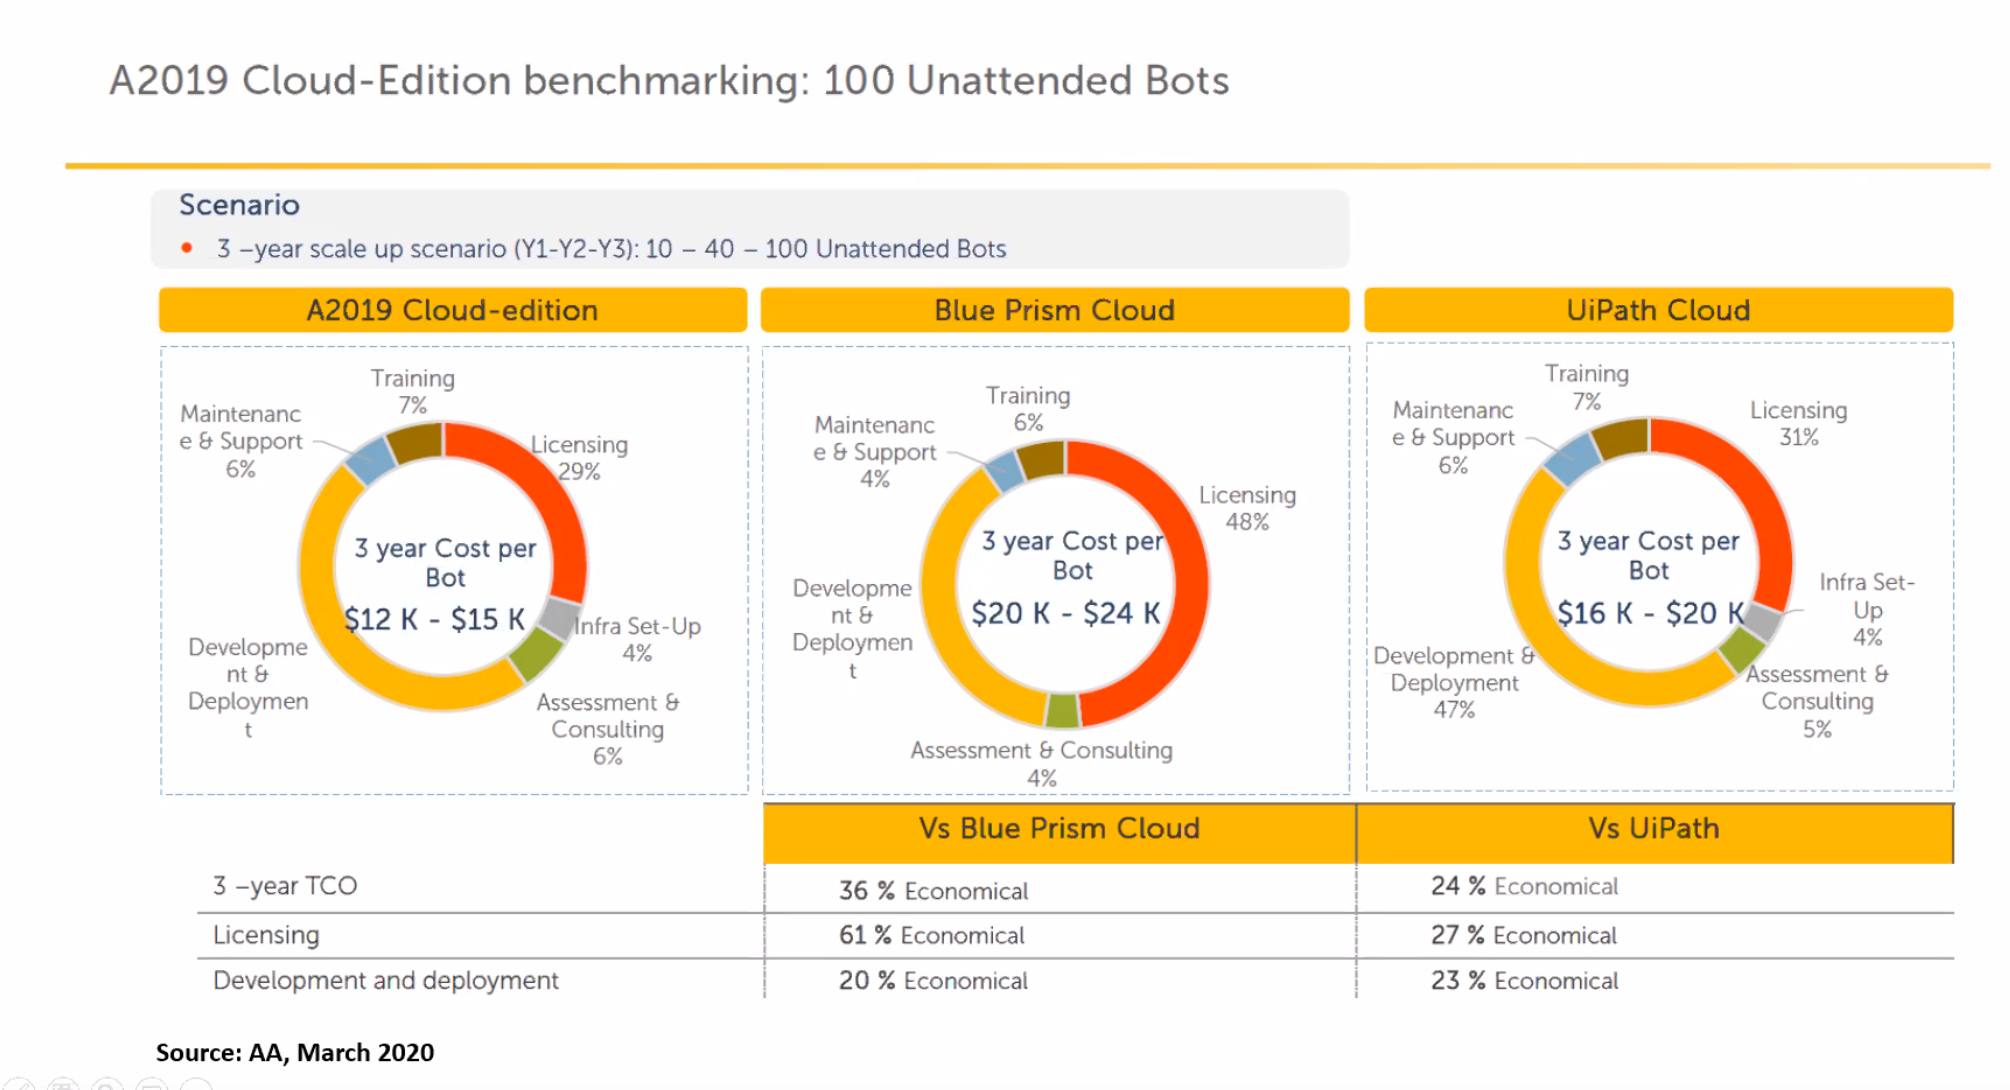
\includegraphics[width=\linewidth]{price_comparison_1.png}
	\caption[Cloud editie benchmarks]{Het verschil in prijs voor een cloud oplossing bij de grote 3 RPA providers.}
	\label{fig:price_1}
\end{figure}
\begin{figure}[h]
	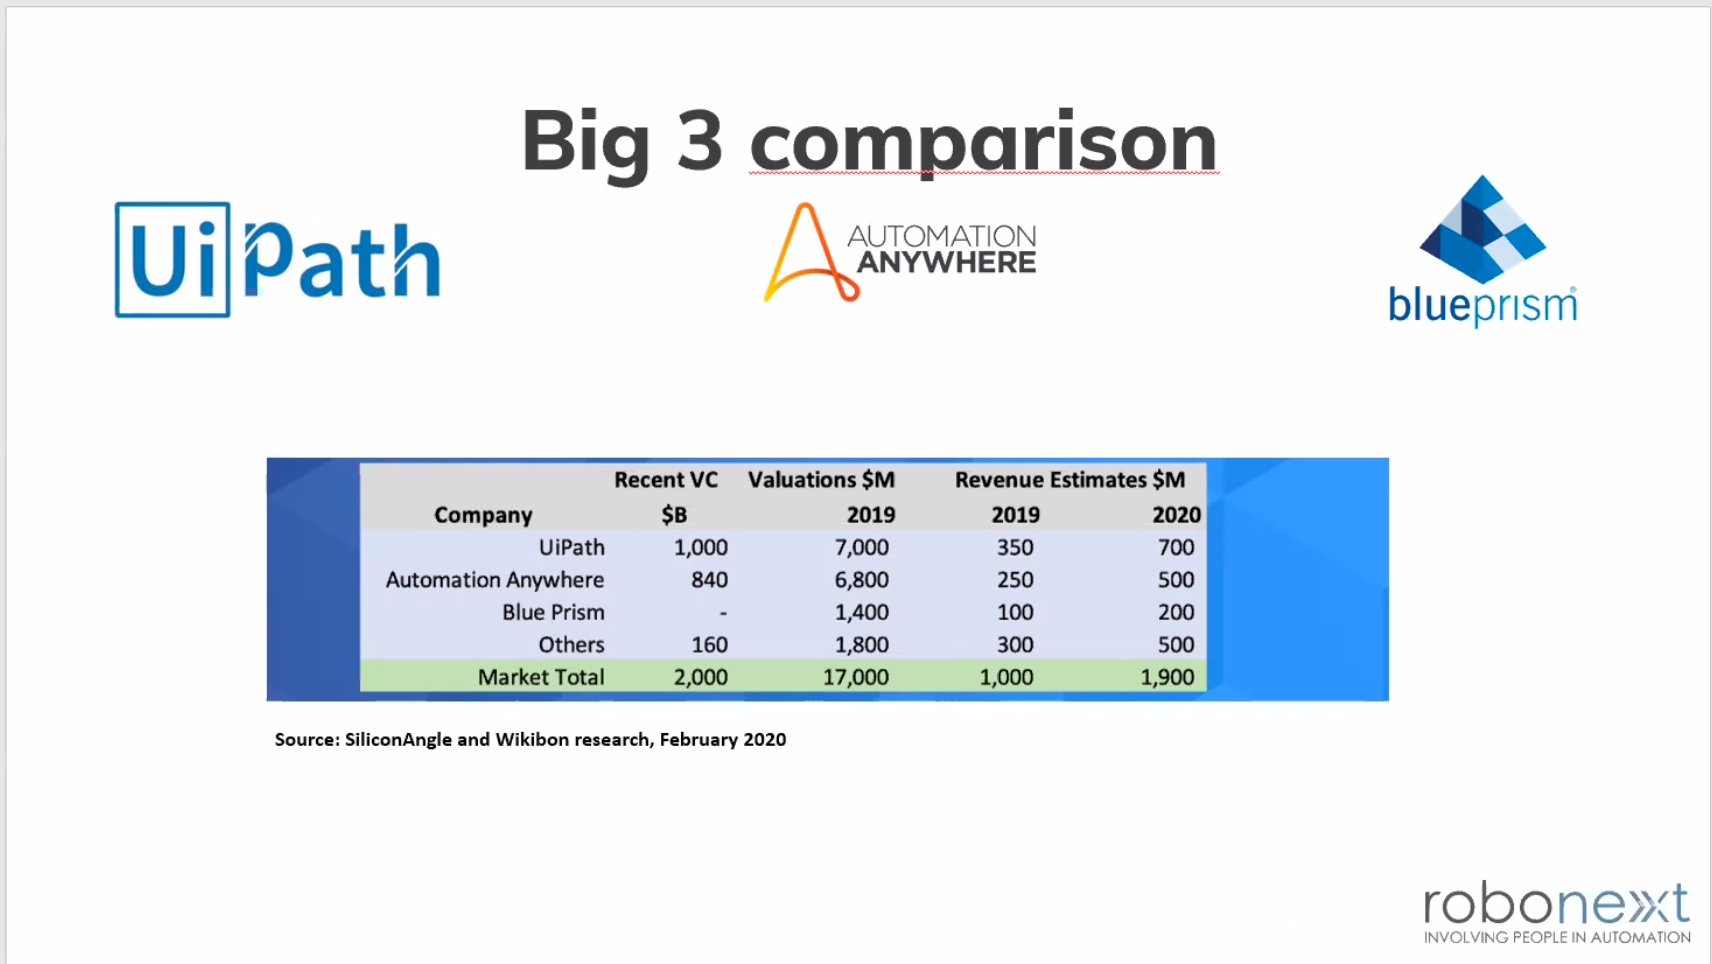
\includegraphics[width=\linewidth]{price_comparison_2.png}
	\caption[Grote 3 Revenue Streams]{Schatting naar marktwaarden en marktaandeel van de grote 3 ten opzichte van de rest.}
	\label{fig:price_2}
\end{figure}
\begin{figure}[h]
	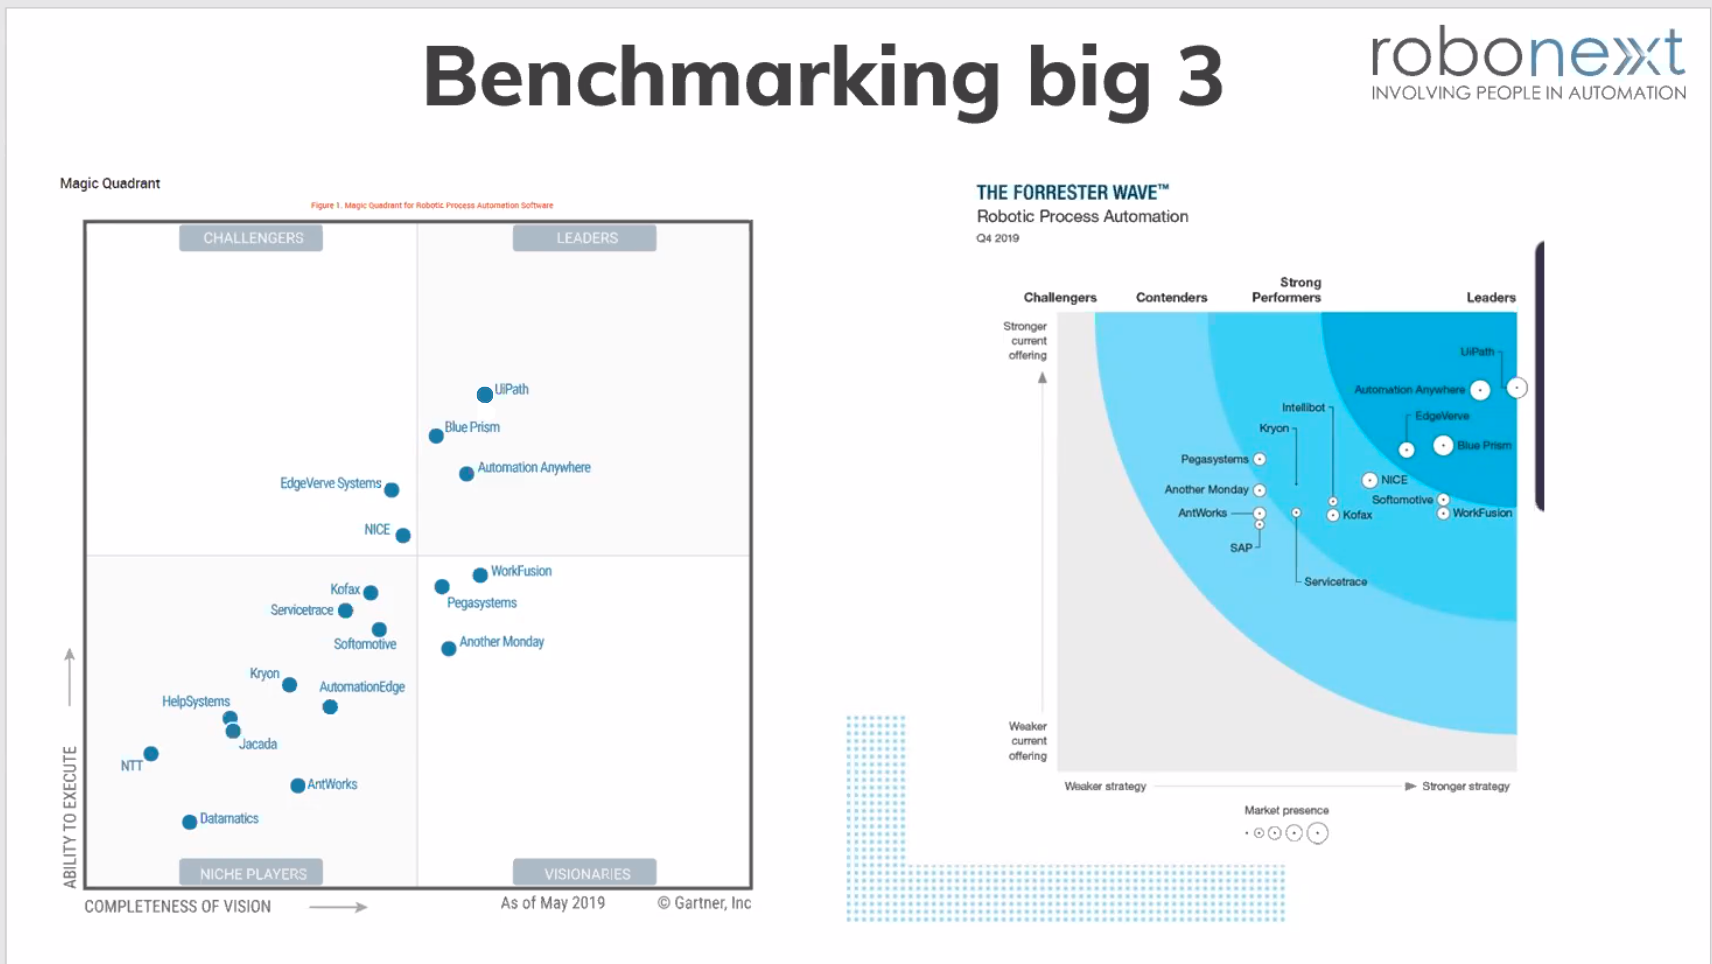
\includegraphics[width=\linewidth]{price_comparison_3.png}
	\caption[Benchmarkings]{De marktleiders en de opkomende spelers.}
	\label{fig:price_3}
\end{figure}